\documentclass[twoside,single]{lion-msc}

\title{Electrochemically changing potential}
\author{Sebastiaan Van Mulken}
\studentid{0950815}
\supervisor{Biswajit Pradhan \\ \hspace*{\fill}Michel Orrit}
\corrector{To be determined}

\begin{document}
\maketitle



\chapter{Introduction}
Since the help of single-molecule fluorescence detection methods, optical studies have made many breakthroughs in the field of science. Single-molecule fluorescence resonance energy transfer (FRET) is one of the most general accepted techniques. Different kind of kinetics of proteins, such as redox switching \cite{Akklc}, have been revealed. In the past, Biswajit Pradhan has taken a closer look at the time traces and autocorrelation of azurin labelled with ATTO 655 under different potentials. Here the potential was changed chemically: different solutions with different concentrations of ascorbate were used to achieve different potentials. The goal of this thesis is to make an experimental set up which can measure the time traces and autocorrelation of single molecules in different potentials. However, a key difference with the set up of B. Pradhan is that the potentials are not changed chemically, but rather electrochemically. With the help of a electrochemical analyser different potentials are achieved. 

In general the setup on its own is meaningless and rather a first step to scientific success. The results are way more important. To discuss the measurements made with the new setup, the autocorrelations of labelled azurin measured with the two different set ups are compared. 
\chapter{Theory}
In this chapter, the fundamental physics and electrochemistry are explained which are used in the set up.

\section{Fluorescence}
Fluorescence is the property of certain atoms and molecules to absorb light at particular wavelengths and emit light at longer wavelengths. These type of atoms and molecules are called fluorophores or fluorescent dyes. A brief interval after absorption - the fluorescence lifetime - the atoms or molecules will emit light of less energy (longer wavelengths).  Fluorescence is a process governed by three events. All these events occur on different timescales separated by several orders of magnitude. These events are summarised in Figure \ref{fluor}.
\begin{figure}[ht!]
\centering
\includegraphics[width=90mm]{fluorescence.jpg}
\caption{The three major events in fluorescence: excitation (1), relaxation (2) and emission (3).} 
\label{fluor}
\end{figure}

\subsection{Excitation}
The first event is excitation. For any molecule, several electronic states exist depending on the total electron energy and the symmetry of the electron spin states. Each state is divided in sub-states - a number of vibrational and rotational energy levels associated with the atomic nuclei and the bonding orbitals. At room temperature, most molecules lack the internal energy to exist in any other state than the lowest vibrational level of the ground state. This ground state is usually an electronic singlet in which all electrons are spin-paired (opposite spins). With the help of a laser, photons with energy $E_{photon}=h \nu_{laser}$ are absorbed by the fluorophores. The absorption of energy happens to any of the closely spaced vibrational and rotational energy levels of the excited states. Absorption of light occurs in a few femtoseconds ($10^{-15}s$). It will only occur for specific wavelengths known as the absorption bands. If a photon contains more energy than necessary for an electronic transition, the excess energy is converted into vibrational and rotational energy via non-radiative processes. If the energy of a photon is too low, no transition occurs. Excitation of a molecule by absorption normally happens without a change in electron spin-pairing. Therefore, the excited state is also a singlet. Usually the fluorophores are excited to higher vibrational levels of the first or second singlet electronic energy state. Certain transitions have higher probability than others and combined they form an absorption spectrum of the molecule.

\subsection{Vibrational relaxation}
After absorption, several processes occur with varying probabilities. The most likely is relaxation to the lowest vibrational energy level of the first excited state, a process known as internal conversion or vibrational relaxation. This is a loss of energy in a non-radiative matter and has a timescale of a picosecond ($10^{-12}s$) or less. Since a significant number of vibration cycles transpire during the excited lifetimes, molecules undergo complete vibrational relaxation. The excess vibrational energy is converted into heat, which is transferred to the neighbouring solvent molecules.

\subsection{Emission}
The excited molecule exists in the lowest excited singlet state for a period in the order of nanoseconds ($10^{-9}s$) before relaxing to the ground state. During this relaxing, a photon will be emitted. Because the ground state consist of closely spaced vibrational energy levels, the resulting emission intensity is distributed over a band of wavelengths rather than a sharp line. Most fluorophores can repeat the excitation and emission cycle a lot of times. However, the excited state is more reactive with the surrounding which can result in photobleaching: the molecule is permanently unable to fluoresce. 

Other relaxation pathways compete with the fluorescene emission process. The excited state energy can be dissipated as heat, the excited molecule can collide with another molecule to transfer energy (for example quenching) or intersystem crossing to the lowest excited triplet state can occur. The latter will result in emission of a photon through phosphorescence or a transition back to the excited singlet state that yields delayed fluorescence. Molecules who exhibit the triplet state have a high degree of chemical reactivity, often resulting in photobleaching. 

\section{Fluorescence Resonance Energy Transfer}
Fluorescence resonance energy transfer (FRET) permits determination of two molecules within several nanometers, the distance close to where molecular interactions occur. The process of resonance energy transfer can take place when the donor fluorophore in an electronically excited state transfer its excitation energy to a nearby chromophore (the acceptor). If the fluorescence emission spectrum of the donor molecule overlaps the absorption spectrum of the acceptor molecule and the two are within minimal spatial radius, the donor can transfer its excitation energy in a non-radiative fashion through dipole-dipole intermolecular coupling. Treating an excited fluorophore as an oscillating dipole, it can undergo energy exchange with a second dipole having a similar resonance frequency. If the acceptor itself is a fluorochrome, increased or sensitised fluorescence emission is observed. By exciting the donor and acceptor molecules with light of wavelengths centred near the absorption maximum of the donor, the detected light will be emitted at wavelengths centred near the emission maximum of the acceptor if FRET has taken place. This resonance energy transfer is not sensitive to the surroundings of a fluorophore. The FRET efficiency is given by:
\begin{equation}
E = \frac{1}{1 + (r/R_{0})^{6}}
\end{equation}
where $r$ is the distance between the donor and acceptor molecule and $R_{0}$ is the F\"oster distance - the distance at which the energy transfer efficiency is 50\%. Related to this efficiency is the lifetime ($\tau_{D}^{'}$ in pressence of an acceptor and $\tau_{D}^{'}$ with the absence of an acceptor) and the fluorescence intensity ($F_{D}^{'}$ in pressence of an acceptor and $F_{D}$ with the absence of an acceptor) via the formulas
\begin{equation}
E = 1 - \frac{\tau_{D}^{'}}{\tau_{D}}
\end{equation}
and
\begin{equation}
E = 1 - \frac{F_{D}^{'}}{F_{D}}.
\end{equation}


\section{FluRedox principles and labelled azurin}
In contrast to FRET, FluRedox is based on the change of the overlap integral associated with a change in the optical properties of the redox-active centre upon oxidation and reduction. This will reduce the chance of abnormal signals from other components in the system, because the optical read-out responds exclusively to the redox state of the protein \cite{Akklc}. 

Azurin is a blue copper protein with an active copper site (see Figure \ref{azurin}). The active centre of azurin has strong characteristic features in its optical absorption spectrum which is dependent on the redox state. It may occur in oxidised ($\textup{Cu}^{2+}$) or reduced ($\textup{Cu}^{+}$) form. Oxidised azurin exhibits a strong absorption band around 600 nm (blue). Fluorescent labelling of this protein makes it suitable for single molecule studies. ATTO-655 is a fluorescence dye with a emission band around 680 nm. When azurin is oxidised, FRET between the dye and the centre quenches the dye fluorescence. This quenching is absent when the protein is in reduced state because its 600 nm absorption has vanished (see Figure \ref{absorption}) \cite{Tabares2014}.

\begin{figure}[ht!]
\centering
\includegraphics[width=50mm]{azurin1}
\caption{Three dimensional structure of azurin. The green sphere is the copper centre of the protein. Picture is taken from \cite{BORMAN2010}.} 
\label{azurin}
\end{figure}

\begin{figure}[ht!]
\centering
\includegraphics[width=90mm]{absorp.jpg}
\caption{Absorption spectrum of $\textup{Cu}^{+}$ (black), $\textup{Cu}^{2+}$ (red) and the emission spectrum of the fluorescence dye ATTO-655 (blue). The absortion band around 600 nm is absent when azurin is reduced.} 
\label{absorption}
\end{figure}


\section{Single molecules techniques}
It is impossible to open newspapers without stumbling over words that reflect the impact of life sciences to the modern world. Many speculations and discussions suffer from vagueness since many biological mechanisms are barely known to exist and even less mechanisms are fully understood. New and more precise techniques have made this field grow quickly. With new synthetic fluorophores, the ability to study single proteins at a time is exploited to investigate a variety of dynamics.  One of the ways to get a better understanding of these single proteins is the usage of fluorescence correlation spectroscopy and the usage of confocal microscopes. 

\subsection{Fluorescence Correlation Spectroscopy}
The instrumentation of Fluorescence Correlation Spectroscopy (FCS) is based on an inverted confocal microscope.  A laser beam is directed into a microscope objective via dichroic mirrors and focused on the sample. High numerical aperture are used, since the sample molecules usually are dissolved in aqueous solution. Fluorescence light from the sample is collected and passed through the dichroic and emission filter. A pinhole in the image plane blocks the light not originating from the focal region. When concentrations in order of a few - or less - nanomolar of fluorescent particles are applied, single particles can be monitored at a given time. A more detailed description can be found in reference \ref{Schwille}.

The fluorescence intensity collected during the experiments were elaborated using the normalized autocorrelation (AC) function, defined by:
\begin{equation}
G'(\tau) = \frac{\left \langle I(t)I(t + \tau) \right \rangle}{\left \langle I(t)\right \rangle ^{2}}.
\end{equation}
Substracting the normal offset of value 1, this leads to
\begin{equation} \label{AC}
G(\tau) = G'(\tau) - 1 =  \frac{\left \langle \delta I(t)\delta I(t + \tau) \right \rangle}{\left \langle I(t)\right \rangle ^{2}}
\end{equation}
where the brackets  denotes temporal averaging and $\delta I(t) = I(t) - \left \langle I(t)\right \rangle$. The autocorrelation function is used to compute the self-similarity after lag-time $\tau$.

\subsection{Confocal Laser Scanning Microscopy}
Confocal Laser Scanning Microscopy (CLSM) is the setup we used in this experiment. The CLSM is used to scan a sample. In contrast to the FCS, the detection of the signal from the sample depends on strategic choices. The sample is mounted on a moving piezoelectric scanning stage. This allows sub-micrometer movements. The scanning stage is moved along the confocal volume and the fluorescent signal is collected for each position sampled. Together with the fluorescence intensity, the setup is equipped to record the lifetime of the fluorescence and time traces with the help of a time-correlated single-photon counting (TCSPC) board. A more detailed description of the setup is found in sections \ref{confo_micro} and \ref{data_coll}.

For this thesis, the Cu-azurin and Zn-azurin were labeled and immobilized on the sample slide. Surrounded by an electron mediator, different potentials were applied on areas of (20 x 20) $\upmu \textup{m}^{2}$, which have around 30 - 40 immobilized proteins. Initially applying a positive and negative potential, by means of lifetime analysis, the working azurin and bleached azurin/impurities can be pointed out directly after taking the images, since the FRET effect affects directly the lifetime of the dye (see Figure \ref{finding_proteins}). Once we select the working proteins, the signal of the proteins is recorded for different time intervals (usually 30 seconds) resulting in time traces as showed in Figure \ref{TT_exam}.

\begin{figure}
\begin{subfigure}{.5\textwidth}
  \centering
  \includegraphics[width=.95 \linewidth]{voorbeeld_protein_2}
  \label{}
\end{subfigure}%
\begin{subfigure}{.5\textwidth}
  \centering
  \includegraphics[width=.95 \linewidth]{voorbeeld_protein_1}
  \label{}
\end{subfigure}
\caption{A  (10 x 10) $\upmu \textup{m}^{2}$  area filled with immobilized Cu-azurin in different potentials. On the left: potential of 100mV, here the Cu-azurin is reduced. The bright spots (red circles) are either bleached proteins or impurities. A way to get rid of these impurities is by focussing the laser with slighty more power on these spots. On the right: same area, but with -100mV potential. All the proteins are oxidised. Comparing these two pictures show inmediately the protein and the impurities.}
\label{finding_proteins}
\end{figure}


\begin{figure}[ht!]
\centering
\includegraphics[width= \textwidth]{TT_example}
\caption{Example of a small part of a 30 sec timetrace of an immobilised Cu-Azurin in a -100mV potential, taken with a CLSM. The blue line is the raw data, the red line is the fitted on and off magnitude and changepoint times. This is calculated using a specific program which is in more detailes described in the Data section.} 
\label{TT_exam}
\end{figure}

\section{Oxidation-reduction reactions}
Electricity is the movement of electrons and can be generated by movements of electrons from one element to another in a oxidation-reduction (redox) reaction. Oxidation is the loss of electrons, reduction is the acquisition of electrons. The species being oxidized is called the reductant and the species being reduced is called the oxidant. The oxidation-reduction reaction can occur spontaneously. This is due to the difference in potential energy between the two substances. This difference is called the cell potential, denoted as $E_{cell}$. This cell potential depends upon the concentration of species as well as temperature. The greater the cell potential the greater is the driving force of the electrons. Since the standard state cell potential $E^{0}_{cell}$ is measured under standard states (1 Molar and 1 atmospheric pressure), it differs from the non-standard state cell potential. The two are closely related via
\begin{equation} \label{nernst}
E_{cell} = E^{0}_{cell} - \frac{RT}{nF} \ln Q
\end{equation}
or in terms of $\log_{10}$
\begin{equation}
E_{cell} = E^{0}_{cell} - \frac{0.0592}{n} \log_{10} Q
\end{equation}
where Q is the reaction quotient. This equation is referred to as the Nernst equation. For a reversible reaction (which is usually the case in redox reactions) $\textup{aA + bB}\rightleftharpoons\textup{cC + dD}$ where a, b, c and d are the stoichiometric coefficients for the balanced reaction, we can calculate the reaction quotient using:
\begin{equation}
Q=\frac{\left [\textup{C}  \right ]^{a}\left [\textup{D}  \right ]^{d}}{\left [\textup{A}  \right ]^{a}\left [\textup{B}  \right ]^{b}}
\end{equation}

\section{Electrochemical detection}
Electrochemical detection instruments can be used for monitoring the current passing through a flow cell in liquid electrochemistry and flow injection analysis, but they can also be used for other electroanalytical applications. The potential control range of these instruments is $\pm10V$. To reach certain potentials, a constant potential is applied and the current is recorded as function of time (amperometric i-t curve), as is shown in Figure \ref{amp_curve}. Once the current in the i-t Curve is constant (i.e flat), the solution has reached the demanded potential. The data sample interval is chosen according to the length of the experiment.

\begin{figure}[ht!]
\centering
\includegraphics[width= \textwidth]{amp_curve}
\caption{The amperometric i-t curve. } 
\label{amp_curve}
\end{figure}

\section{Binding protein to the surface}\label{neutra}
In a variety of different applications the biotin-avidin system has been used \cite{Diamandis1991}. Living organisms develop highly specific defence mechanisms to help survive in unfriendly environments. Avidin, a protein found in egg white, has the ability to bind with very high affinity to vitamin biotin. This interaction is thought to represent the natural defence mechanism: the binding of avidin with biotinylated enzymes inactivates the enzymes.and thus inhibits the growth of bacteria. Compared to other  ligand-binder interactions, biotin-avadin has unique characteristics. The nonconvalent interaction of avadin with biotin has a formation constant of $10^{15}\textup{L}\cdot \textup{mol}^{-1}$, much greater than the interaction of ligands with their specific antibodies (about $10^{3}-10^{6}$ times greater). Also the avidin to biotin binding is specific enough to ensure the binding direct to the target of interest. Finally, the avidin possesses four binding sites per molecule. 

The NeutrAvidin is used unlabeled and serves as a link between the biotinylated binder (the biotin on the glass slide) and the biotinylated molecule (labeled Cu-azurin). This is illustrated in Figure \ref{avadinbinding} 

\begin{figure}[ht!]
\centering
\includegraphics[width=70mm]{avadin}
\caption{Illustration of the sample slide - NeutrAviding - protein binding. The red cross is the NeutrAvidin, with the four corners representing the binding spots for biotin. The yellow rectangulars represent the biotin. One side is bound to the glass surface while the other side is connected to the azurin}
\label{avadinbinding}
\end{figure}

\chapter{Set-up}

In this chapter the road to the final experimental set-up is explained in detail. It is divided in three parts: the first part describes the previously used set-up. This set-up change the potential chemically. The second part of this chapter shows the progress from scratch to the final set-up including the things that did and did not work. In papers and publications, it is not  common to describe how the experiment was built from the start till the end, but it is sufficient to describe this in more detail since it took more than the usual time for a bachelor thesis. The final part of this chapter describes the final set-up, with which the data we discuss later is acquired. 

Before we discuss the old set-up, we start with the basics that were used in both set-ups.  

\section*{Confocal microscope}  \label{confo_micro}
To perform the experiment, a home built confocal microscope used previously for similar experiments \cite{Gupta2014} was used. A 639 nm pulsed laser, controlled by a PDL 800-B (PicoQuant) laser driver at 40MHz repetition rate, is passed through a narrow band filter (LD01-640/8-25, Semrock). To collimate the beam to the desired diameter an aspheric lens of suitable focal length was used. The beam then got reflected via a dichroic mirror (ZT640RDC, Chroma) to the high numerical aperture (NA) oil immersion objective (1.4 NA, 100X oil, Zeiss). The stage on which the sample was mounted was controlled by a nanopositioning piezo element (P517.3CD, Physic Instrumente). The emission was collected and filtered through an emission filter (ET655LP, Chroma) and focused onto a $50\upmu \textup{m}$ pinhole to filter the background. Once the beam got focused on the active area of a single photon counting module (SPCM-AQR-14, Perkin Elmer) data acquisition was performed by a photon counting PC-board (TimeHarp 200 PicoQuant). A schematic set up is shown in Figure \ref{micros}.

\begin{figure}[ht!]
\centering
\includegraphics[width=70mm]{schem_micros}
\caption{Schematic drawing of the confocal microscope used in the chemical and electrochemical set up.}
\label{micros}
\end{figure}


\section*{Functionalizing glass slides}
Not only the same confocal microscope was used in both set-ups, also the immobilization of the proteins is similar. The functionalization of the cover glass is based on the process used in \cite{Gupta2014}.  \diameter 25mm \#1 thickness glass coverslips (Menzel-Glaser) were used for all immobilizations. The coverslips were rinsed several times with milliQ water and treated with a  $\textup{H}_{2}\textup{O} / \textup{NH}_{4}\textup{OH} / \textup{H}_{2}\textup{O}_{2}$ (5:1:1) bath at 70 \degree C. The coverslips were then rinsed again but with water and finally with ethanol. The result of this process is the coverslips contain active silanol groups which can react with silanes and thus providing capability to functionalize the surface. The coverslips were stored in ethanol.


Before usage, the coverslips were flamed and then ozone cleaned for 15 minutes. Then the coverslips were treated for 30 min with a 1\% solution of 3-(2-aminoethyl)aminopropyl trimethoxysilane in methanol containing 5\% glacial acetic acid. After washed extensively with methanol, the coverslips were sonicated with intervals of 10 minutes. Dried with clean nitrogen, it was left in the desiccator overnight or kept in the oven at 65 \degree C for 3 hours. The next day they were treated with a 5 mg/ml solution of methoxy-peg-NHS (MW 2000, Laysan Bio) and biotin-peg-N-hydroxysuccinimide (MW 3400, Laysan Bio) in 50mM sodium phosphate buffer (pH 8). To ensure enough biotin functionalities are present the ratio of biotin peg to methoxy was kept at 1:10.  






\section{Changing the potential chemically}\label{pot_chem}

\begin{figure}[ht!]
\centering
\includegraphics[width=70 mm]{old_setup}
\caption{Schematically representation of the chemically induced experiment.*** Need to change picture***}
\label{old_setup}
\end{figure}

A schematically picture of the set-up can be seen in Figure \ref{old_setup}. A small glass slide is functionalised in a similar way explained previously. A syringe is used to suck solution through the tubes onto the glass slide. One side is connected to the syringe, the other side is connected to the desired solution. First a mixture of proteins is put on the glass slide. After sufficient time, the proteins will bind to the glass slide. A new mixture consistent of buffer HEPES (pH = 7) is then sucked through the tube onto the glass slide to remove non-bound proteins. Once the proteins are removed, a new mixture consistent of ascorbate ($\textup{C}_{6}\textup{H}_{8}\textup{O}_{6}$) is put on one end. Ascorbate is an antioxidant and exists prediminantly as the ascorbate monoanion  $\textup{AschH}^{-}$. The standard potential of ascorbate is 0.282mV (pH = 7), which is close to the standard potential of the proteins. Oxidation of ascorbate forms $\textup{ascorbyl radical Asc}^{\bullet  -}$, the equivalent of ascorbate but with one less proton and one less electron. Upon further oxidation this becomes dehydroascorbate ($\textup{C}_{6}\textup{H}_{6}\textup{O}_{6}$) \cite{Warren2010}. Schematically this becomes:

\begin{figure}[ht!]
\centering
\includegraphics[width=\textwidth]{redox_asc}
\caption{Redox of ascorbate}
\label{redox_asc}
\end{figure}

At equilibrium, using the Nernst equation (Formula \ref{nernst}), the potential can be written as

\begin{equation}
E = E^{0}_{Asc} - \frac{RT}{F} \log_{10} \frac{[\textup{C}_{6}\textup{H}_{6}\textup{O}_{6}]}{[\textup{C}_{6}\textup{H}_{8}\textup{O}_{6}]}.
\end{equation}

Thus by adjusting the concentration of ascorbate (in this case adding ascorbate), different potentials will be achieved in the solution. The final redox potentials of the solution were measured with a reference electrode (standard calomel, SCE) and a platinum counter electrode connected to a voltmeter.

\section{Process to the final set-up}

The previous set-up based the redox switching on chemically induced changes. In the new set-up, these changes are achieved electrically. Beside the confocal microscope, a new instrument has to be introduced: the electrochemical analyzer (Model 800B Series Electrochemical Detector, CH Instruments). Instead of using different concentrations of ascorbate, a cell with a working electrode, counter electrode and reference electrode in a buffer is used. During the process of getting to the final set-up, the same working electrode, counter electrode and reference electrode is used: a \diameter250mm golden wire acts as the working electrode, the counter electrode is a \diameter0.5 mm thin platinum wire and the reference electrode is a saturated calomel electrode. All the potentials throughout this work are reported relative to the SCE.

\subsection{Electron mediator}\label{ferriferro}
When looking at single molecule level, it is expected to see the molecule spend half the time reduced and half of the time oxidized when the potential is set to the mid-point potential of the molecule. This  is evidenced by equal on- and off-times for the blinking. For reducing potentials the molecule will spend more time in the off state and for oxidizing potentials the molecule will spend more time in the on state. It is therefor important to have a range of potentials that are below and above the mid-point potential of the molecule of interest. In the case of Cu-azurin, the midpoint potential is around ... mV. A solution consistent of a buffer and a redox-pair is needed to act as a electron mediator to obtain the potentials around the mid-point potential of Cu-azurin. A good way to check what range of potentials such solution can reach is the use of cyclic voltammetry (CV) measurement. This is a plot of the current versus the potential. Since the previous set-up did not use the potentiostat, the first thing we did for this experiment was using this device to obtain the CV of different solutions to find the one solution that suits this experiment the best.

To obtain the CV of different solutions, a small set-up was made. A volume of around 200mL was put on top of magnetic mixer and the working, reference and counter electrode were lowered into the solution and connected to the electrochemical analyzer. With this set-up, three different solutions were tested to see which would obtain the best results. 
\begin{enumerate}
\item A solution with ascorbate which is used in the chemically-induced redox switching set-up. The details of the redox of ascorbate is described in more detail in section \ref{pot_chem}.
\item With a midpoint potential of $-237 mV$, the redox couple potassium ferricyanide ($[\textup{Fe(CN)}_{6}]^{4-}$)/ferrocyanide ($[\textup{Fe(CN)}_{6}]^{3-}$) is an almost perfect canditate for this experiment. The oxidation of ferrocyanide, resulting in ferricyanide is given by
\begin{equation}
[\textup{Fe(CN)}_{6}]^{4-}\rightleftharpoons[\textup{Fe(CN)}_{6}]^{3-} + \textup{e}^{-}.
\end{equation}
Following the Nernst equation:
\begin{equation}
E = E^{0}_{\textup{FeCN}} - \frac{RT}{F} \log_{10} \frac{[\textup{Fe(CN)}_{6}]^{3-}}{[\textup{Fe(CN)}_{6}]^{4-}}.
\end{equation}
In the final set-up, the total volume of the solution is 4 mL. When tried to measure the potential of the ferri/ferro redox couple, a volume of 200-300mL was used. While stirring, oxidizing the redox couple was a fast process. Reducing the ferricyanide, however, took much longer. A possible explanation could be oxidative stress. An explanation could be oxidative stress. Water contains hydrogen in the oxidation state +1 and oxygen in the oxidation state -2. Because of that, the reaction
$$\textup{Fe}^{3+}+\textup{O}_{2}^{-}\rightarrow\textup{Fe}^{2+}+\textup{O}_{2} $$
can occur \cite{Grady1991}. This will slow down the production of $\textup{Fe}^{3+}$ and thus according to the Nernst equation, lower potentials will be reached slower or not at all. Also the set-up is not sealed from the air which contains oxygen. In previous voltage-induced redox switching experiments, only measurements in anaerobic conditions were performed \cite{Akkilic2015}. 
\item Phenazine ethosulfate (PES).
\end{enumerate}
Since there were some issues with the ferricyanide and ferrocyanide redox couple during the very first experiments, we decided to use for the first few experiments PES as the electron mediator. PES in oxidized state may receive electrons from the electrode to get reduced. During the experiments the molecules were very close to the working electrode and in this closed vicinity the redox potential is controlled by the concentration ratio of $\textup{[PES]}_{ox}/\textup{[PES]}_{red}$. This ratio is - on its own term - determined by the potential applied on the working electrode.

\subsection{Proteins on the surface}
Having functionalized sample slides and a fitting electron mediator, the next phase in the process to the final set-up is to get the right amount of proteins on the sample slide. As mentioned in section \ref{neutra},  NeutrAvidin is used as a link between the sample slide and the proteins and has four possible bind spots  (Figure \ref{avidinratio}). Before the proteins were applied on the sample slide, they were mixed together with the NeutrAvidin. Different ratios between proteins and NeutrAvidin were tried to find the right ratio. When more proteins bind to the same NeutrAvidin, the proteins will quench due to collisional quenching. The quencher diffuses to the protein during the lifetime of the excited state. Upon contact, the proteins returns to the ground state, without emission of a photon. The protein and quencher must be in contact \cite{Lakowicz2006}. The quenching proteins visualizes as blue spots on the sample slide, as is clearly the case when the ratio between proteins and NeutrAvidin was 1:1 (see Figure \ref{finding_proteins}). Lowering the ratio of proteins to the same amount of NeutrAvidin ensures the fact that less protein will bind to the same NeutrAvidin untill the point that almost all of the NeutrAvidin has only one binding to the surface. This is the case when the ratio between protein and NeutrAvidin 1:40 (Figure \ref{1:40}). This is the ratio that is used in further experiments.

\begin{figure}[ht!]
\centering
\includegraphics[width=70mm]{ratio_avadin}
\caption{Illustration of NeutrAvidin (red cross) bound to three azurin molecules via biotin (yellow). This is likely the cause of collisional quenching.}
\label{avidinratio}
\end{figure}


\begin{figure}
\begin{subfigure}{.5\textwidth}
  \centering
  \includegraphics[width=.95 \linewidth]{onetooneratio}
  \label{}
\end{subfigure}%
\begin{subfigure}{.5\textwidth}
  \centering
  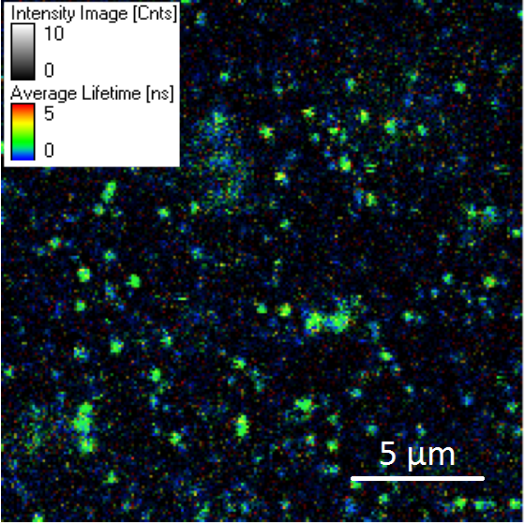
\includegraphics[width=.95 \linewidth]{onetofive}
  \label{}
\end{subfigure}
\caption{A (20 x 20) $\upmu \textup{m}^{2}$ image of immobilised azurin on the sample slide with different ratios of protein to NeutrAvidin. Left: the ratio between protein and NeutrAvidin is 1:1. Right: the ratio between protein and NeutrAvidin is 1:5. When the amount of proteins to NeutrAvidin is decreased, a decreased amount of quenched proteins (blue spots) is observed.}
\label{finding_proteins}
\end{figure}


\subsection{The working electrode}
In an electrochemical system, the working electrode is the electrode of interest. In this case the working electrode is made of gold, since gold is one of the best electron conductors. The reaction of interest is occurring on and near the working electrode in conjunction with the counter electrode and reference electrode. Since the establishment of the redox potential relies on the diffusion of the electron mediator, the actual redox sensed by the molecule is dependent on the distance between the working electrode and the molecule as well as on the time after an external potential is applied. One way to keep the distance between the molecule and working electrode as small as possible is by creating a gold layer on top of the functionalized sample slides with the help a sputtering machine. This gold layer is in touch with the electrochemical analyzer via a \diameter250mm golden wire.  By creating transparent areas where proteins are immobilized such that the distance between the gold border and proteins are sufficient small and assuring to apply an external potential long enough, it can be assumed that the potential on the gold is equal to the one in the near surrounding. Using a 20nm gold layer gave a lot of problems, however. 

One of the problems to overcome was to find a proper way to create transparant areas in the gold. Several different methods were tried (see Figure \ref{gold_layer}) and some of them are described hereafter.
\begin{enumerate}
\item \textbf{Scratches}.  The first attempt was sputtering the whole glass slide with a 20 nm layer of gold. With a needle scratches were made and imaged. When making scratches it is of big importance to not cross other scratches. Once the scratches cross each other, areas of gold that are isolated from the goldlayer that is in touch with the wire can be created. The gold will not be connected to the working electrode in that case and no electrochemical changes will be seen near those edges. Once the scratches were made and put under the microscope it was easy to locate the transparent areas. However, the transparent areas created in this way were often too small for single molecules experiments. Beside that, the functionalised sample slide happened to get damaged along this process: when making scratches it is difficult to apply the same pressure along the scratches resulting in different depth of scratches. The dimension of proteins are in the nanometers. Different deepness make it impossible to focus on multiple proteins in the same area at once.
\item \textbf{Small pieces of glass.} To get areas with the same depth, small pieces of smashed glass were laying on top of the immobilised glass slide before they were sputtered with gold. Once the sputtering was finished, the pieces of glass were removed resulting in small transparent areas (see the leftside of Figure \ref{gold_layer}). The borders between glass and gold were sharp (the borders were 'slim' on the images), but again a lot of very small - and thus useless to image multiple proteins in an area - areas were formed via this method. Later it was done with only a few bigger pieces of glass to avoid these small areas. This showed some improvement. 
\item \textbf{Metal crosses.} Small metal crosses on top of the glass before sputtering, resulting in cross-like transparant areas (see Figure \ref{gold_layer}). These transparent areas were easy to locate, the edges were straight and the borders were sharp as long as the gold layer was 30 nm thick, see Figure \ref{border}. If a certain (80 x 80) $\upmu \textup{m}^{2}$ area didn't suit single protein experiments, it is easy to slide along the border to find an area that suits better. 
\end{enumerate}

\begin{figure}
\begin{subfigure}{.5\textwidth}
  \centering
  \includegraphics[width=.7\linewidth]{glass}
  \label{cross}
\end{subfigure}%
\begin{subfigure}{.5\textwidth}
  \centering
  \includegraphics[width=.7\linewidth]{cross}
  \label{glass}
\end{subfigure}
\caption{A few examples of the \diameter 25mm glass slides with a golden layer on top of it. Left: the transparent areas created with the help of small pieces of glass. Right: with the use of small iron crosses a transparent area with the form of a cross was created.}
\label{gold_layer}
\end{figure}

\begin{figure}[ht!]
\centering
\includegraphics[width=\textwidth]{border_legenda}
\caption{(80 x 80) $\upmu \textup{m}^{2}$ image of the slim border. The top part of the image is gold, the bright blue line is the border between the gold and the glass and the green spots below the border is azurin.}
\label{border}
\end{figure}

The latter method to create reliable areas is used in the next phase of the experiment: the combination of the electron mediator, proteins and the gold layer. Individually these parts worked as intended. However, a combination of the parts lead to two serious problems:
\begin{enumerate}


\item Damaged gold layer.
The longer the experiment continued, the more clear it was that the border of the goldlayer would slowly seperate. At the end of a day of experiments, the gold layer was damaged to such an extend that it would simply seperate from the sample slide. The PES is most likely the reason for this. Though the exact reason for this was never clear - when a golden layer was exposed to a different electron mediator (ferricyanide or ascorbate) the gold layer seemed to be not damaged. The damage caused by PES can be seen if you compare the border of the gold layer (bright blue) of Figure \ref{no_prot} - taken at the start of the experiment -  with the border of Figure \ref{damaged_border} (this picture was taken towards the end of a day of experiments). One way to tackle this problem, as suggested by one of the professors, would be a protective layer on top of the gold layer. This protective layer is the substance .. . This kind of protective layer has been used in similar experiments \cite{Elmalk2012} where it has been shown that the length of the carbon chain can vary without effecting the electron exchange between the gold and the single molecule. In these experiments, however, usually the molecules were on top of the gold layer whereas in our case the proteins are next to the gold layer. The result of using this protective layer was that the proteins did not show any redox, even when different potentials were applied. Since the protective layer did not work, the other way to tackle the damaged gold layer is an increase in thickness of the gold layer. This will not solve the problem, but delay it long enough to do proper experiments. In all previous experiments, the thickness of the gold layer was 20nm. Increasing the thickness of the gold layer led to the second problem.

 \begin{figure}[ht!]
\centering
\includegraphics[width=\textwidth]{damagedborder}
\caption{(80 x 80) $\upmu \textup{m}^{2}$ of the bright blue border between gold (far right) and glass (left), showing the fractured border due to PES damaging the golden layer.}
\label{damaged_border}
\end{figure}

\item Missing proteins.
Near the edges of the working electrode, a much lower density of proteins was observed (see Figure \ref{no_prot}) once the gold layer thickness was increased. The reason for this could be that during the sputtering of the gold layer, the metal crosses would slightly move a little bit and thus damaging the methoxy-peg-NHS layer. This would make it harder for proteins to bind near the surface. Another explanation could be the fact that some gold-particles might have slipped under the metal cross and taking the spots where the proteins usually would bind. A final explanation would be something with the plasma (need to look at this Bis).


\begin{figure}[ht!]
\centering
\includegraphics[width=\textwidth]{no_prot}
\caption{The (80 x 80) $\upmu \textup{m}^{2}$ of the glass surface near the 200nm thick golden layer. As can be seen, almost no proteins are present despite using the same molecule densities.}
\label{no_prot}
\end{figure}

\end{enumerate}

\subsection*{The final set-up: platinum grid} \label{grid_1}
At this point of the process it was clear that the gold-layer as a working electrode in the current set-up gave too many problems and a final solution was attempted. Instead of using a gold layer, a single golden wire was kept on the sample slide to see if this would give any good results. This can be seen in Figure \ref{goldenwire_1}. The green color are the proteins showing switching and blinking. This was the first sign that instead of the golden layer, a (golden) wire as working electrode could do the trick.  Finding a single wire with the microscope and keeping it on the sample slide is a tough task and is not controllable. Instead of one golden wire, a platinum grid is used and pressed on the sample slide. This grid has a thickness of ...  and sides of (200 x 200)nm (need to find proper dimensions). When using the platinum grid, redox of the proteins is visible, as can be seen in Figure \ref{finding_proteins}. This was the last step in order to have the whole set-up work as intended. The set-up is schematically drawn in Figure \ref{final_setup} with a short description of the parts.


\begin{figure}[ht!]
\centering
\includegraphics[width=\textwidth]{goldwire_1}
\caption{A (80 x 80) $\upmu \textup{m}^{2}$ area of the sample slide with immobilized proteins. The blue 'snake' is the golden wire that touches the sample slide. The green spots represent the oxidized proteins. This is the first proof that proteins near the wire show oxidation.}
\label{goldenwire_1}
\end{figure}



\begin{enumerate}
\item The confocal miscrope as described at the begining of this chapter.
\item The\diameter 25mm \#1 thickness functionalized sample slides, also described in detail at the start of this chapter.
\item Solution of ferricyanide and ferrocyanide. Details in section \ref{ferriferro}.
\item The working electrode in connection with the grid (section \ref{grid_1}).
\item The Saturated calomel electrode, functioning as the reference electrode.
\item A platinum wire, not touching the grid, as the counter electrode.
\item The electrochemical analyzer ( Model 800B Series Electrochemical Detector, CH Instruments).
\item Top view of the sample slide. The proteins are not shown in this picture.

\end{enumerate}


\begin{figure}[ht!]
\centering
\includegraphics[width=\textwidth]{final_setup}
\caption{The final set-up for the electrically induced redox switching. The numbers are explained in the text. This figure is not on scale.}
\label{final_setup}
\end{figure}



\chapter{Results and discussion}

\section*{Data collection} \label{data_coll}
The sample, mounted on the scanning stages, was brought into the focal plane of the objective. To find the wire on the surface, images of (80 x 80) ($\upmu \textup{m}^{2}$) were recorded as x-y scans. Once the wire was located, a positive and negative potential is applied and captured to detect the blinking molecules. Images of typically (20 x 20) ($\upmu \textup{m}^{2}$) were recorded in which at least 10 blinking molecules were present. To collect data from a single molecules, the laser was parked on the blinking molecule and measurements were made for 60 seconds. Once all the blinking molecules of interest were measured, a new potential was applied and this process repeated. Many fluorophores bleach within seconds, thus only the time traces of those molecules who survived all the different potentials were included for further analysis. 

To make sure that the surroundings of the singe molecules were indeed the intended potential, the I-t curves were recorded at the same time.


\section*{Time trace analysis}
The software used for the fluorescence lifetime imaging and correlation software is SymPhoTime 64. With the help of this program, timetraces and its specific parameters are saved in .pt3 files. Older versions of SymPhoTime saved this data into .t3r files. Previous PhD student .. had written a program in MATLAB R2012b and C++ to read out the .t3r files and transfer the timetraces into multiple .dat files. This program has been adjusted in such a way it can read out the .pt3 files from the newer version of SymPhoTime 64. It allows you to manually select parts of the timetrace, as is shown in Figure \ref{timetrace_selection}.

\begin{figure}[ht!]
\centering
\includegraphics[width=\textwidth]{timetrace_selection}
\caption{Selection of a timetrace with a program written in MATLAB R2012b and C to select the parts of the timetrace (in red) that will be put into .dat files. As in this specific case the Cu-Azurin bleached around 25.7 second mark and the timetrace once it is bleached is not of interest and therefore not selected.}
\label{timetrace_selection}
\end{figure}

Once the timetrace is selected and put into several .dat files, another C program is run to precisely calculate the  on- ($\tau_{on}$) and off times ($\tau_{off}$) of a specific protein. This program uses a special method to analysis optical single molecule emission data that exhibit discrete intensity jumps, as has been described by Lucas P. Watkins and Haw Yang \cite{And2004}. The program they have written allows precise location of intensity jumps as is shown in Figure \ref{on_off_times}. The on- and off-times are also visualised here. These times are defined as the duration of the proteins being oxidised ($\tau_{on}$) and reduced ($\tau_{off}$).

Looking at the timetraces a trend is noticable on sight. For the higher potentials, the $\tau_{off}$ are long and the $\tau_{on}$ are relatively short which goes hand in hand with the lower amount of events. When the potential decreases towards $25mV$, the amount of events start to increase and the $\tau_{on}$ becomes longer while $\tau_{off} shorter$. This is shown in Figure \ref{25-50m} and Figure \ref{25-50m}. When the potential is coming closer to $0mV$, instead of longer on-times, smaller on-times on quick succession are noticed where-as longer on-times are expected. This is illustrated in Figure \ref{} where a timetrace of $15 mV$ is shown with an more expected $\tau_{on}$ and $\tau_{off}$ fit. These short on-times are not because of the switching between reduced and oxidiced of the single molecule but because of the blinking of the dye.

\begin{figure}[ht!]
\centering
\includegraphics[width=\textwidth]{on_off_test1}
\caption{Same timetrace as Figure \ref{timetrace_selection} but a smaller range. In red is plotted the calculated intensity jumps according to the program written by Lucas P. Watkins and Haw Yang. The time when the intensity is low is refered to as the $\tau_{off}$ and the time the molecules intensity is high is the $\tau_{on}$.}
\label{on_off_times}
\end{figure}


\begin{figure}
\centering
   \begin{subfigure}[b]{1\textwidth}
   \includegraphics[width=0.85\linewidth]{timetrace_plus_fit_25mV}

\end{subfigure}

\begin{subfigure}[b]{1\textwidth}
   \includegraphics[width=0.85\linewidth]{timetrace_plus_fit_50mV}

\end{subfigure}

\caption{Plot of the raw data with the fit (calculated by the change-point program written by Lucas P. Watkins and Haw Yang) of the same molecule exposed to a potential of 25mV and 50mV.}
\label{25-50mV}
\end{figure}

\begin{figure}
\centering
   \begin{subfigure}[b]{1\textwidth}
   \includegraphics[width=0.85\linewidth]{timetrace_plus_fit_75mV}

\end{subfigure}

\begin{subfigure}[b]{1\textwidth}
   \includegraphics[width=0.85 \linewidth]{timetrace_plus_fit_100mV}

\end{subfigure}

\caption{Plot of the raw data with the fit (calculated by the change-point program written by Lucas P. Watkins and Haw Yang) of the same molecule exposed to a potential of 75mV and 100mV.}
\label{75-100mV}
\end{figure}




\iffalse

\begin{figure}
\centering
\includegraphics[width=\textwidth]{2dhistograms_0mV}
\caption{Histogram of the on and off times of Cu-Azurin in a 0 mV potential.}
\label{2dhistograms_00mV}
\end{figure}

\begin{figure}
\centering
\includegraphics[width=\textwidth]{2dhistograms_10mV}
\caption{Histogram of the on and off times of Cu-Azurin in a 10 mV potential.}
\label{2dhistograms_0mV}
\end{figure}

\begin{figure}
\centering
\includegraphics[width=\textwidth]{2dhistograms_15mV}
\caption{Histogram of the on and off times of Cu-Azurin in a 15 mV potential.}
\label{2dhistograms_0mV}
\end{figure}

\begin{figure}
\centering
\includegraphics[width=\textwidth]{2dhistograms_20mV}
\caption{Histogram of the on and off times of Cu-Azurin in a 20 mV potential.}
\label{2dhistograms_0mV}
\end{figure}

\begin{figure}
\centering
\includegraphics[width=\textwidth]{2dhistograms_25mV}
\caption{Histogram of the on and off times of Cu-Azurin in a 25 mV potential.}
\label{2dhistograms_0mV}
\end{figure}

\begin{figure}
\centering
\includegraphics[width=\textwidth]{2dhistograms_35mV}
\caption{Histogram of the on and off times of Cu-Azurin in a 35 mV potential.}
\label{2dhistograms_0mV}
\end{figure}

\begin{figure}
\centering
\includegraphics[width=\textwidth]{2dhistograms_40mV}
\caption{Histogram of the on and off times of Cu-Azurin in a 40 mV potential.}
\label{2dhistograms_0mV}
\end{figure}

\begin{figure}
\centering
\includegraphics[width=\textwidth]{2dhistograms_45mV}
\caption{Histogram of the on and off times of Cu-Azurin in a 45 mV potential.}
\label{2dhistograms_0mV}
\end{figure}

\begin{figure}
\centering
\includegraphics[width=\textwidth]{2dhistograms_50mV}
\caption{Histogram of the on and off times of Cu-Azurin in a 50 mV potential.}
\label{2dhistograms_0mV}
\end{figure}

\begin{figure}
\centering
\includegraphics[width=\textwidth]{2dhistograms_55mV}
\caption{Histogram of the on and off times of Cu-Azurin in a 55 mV potential.}
\label{2dhistograms_0mV}
\end{figure}

\begin{figure}
\centering
\includegraphics[width=\textwidth]{2dhistograms_60mV}
\caption{Histogram of the on and off times of Cu-Azurin in a 60 mV potential.}
\label{2dhistograms_0mV}
\end{figure}

\begin{figure}
\centering
\includegraphics[width=\textwidth]{2dhistograms_65mV}
\caption{Histogram of the on and off times of Cu-Azurin in a 65 mV potential.}
\label{2dhistograms_0mV}
\end{figure}

\begin{figure}
\centering
\includegraphics[width=\textwidth]{2dhistograms_75mV}
\caption{Histogram of the on and off times of Cu-Azurin in a 75 mV potential.}
\label{2dhistograms_0mV}
\end{figure}

\begin{figure}
\centering
\includegraphics[width=\textwidth]{2dhistograms_85mV}
\caption{Histogram of the on and off times of Cu-Azurin in a 85 mV potential.}
\label{2dhistograms_0mV}
\end{figure}

\begin{figure}
\centering
\includegraphics[width=\textwidth]{2dhistograms_90mV}
\caption{Histogram of the on and off times of Cu-Azurin in a 90 mV potential.}
\label{2dhistograms_0mV}
\end{figure}

\begin{figure}
\centering
\includegraphics[width=\textwidth]{2dhistograms_100mV}
\caption{Histogram of the on and off times of Cu-Azurin in a 100 mV potential.}
\label{2dhistograms_100mV}
\end{figure}

\subsection{Average on and off times}
As can be seen from the timetraces, a range of different $\tau_{on}$ and $\tau_{off}$ are visible in a single timetrace. Assuming they should be more or less the same, the average is taken. This leads to one  $\tau_{on}$ and one $\tau_{off}$ for each protein. This is plotted in Figure \ref{Cu_all_times}. 

\begin{figure}
\centering
\includegraphics[width=\textwidth]{Cualltimes1}
\caption{Plot of the on and off times for different Cu-Azurin. Some Cu-Azurin survived more different potentials than others before they bleached. This results in different amount of on and off times for each potential. }
\label{Cu_all_times}
\end{figure}



\begin{figure}
\centering
\includegraphics[width=\textwidth]{ZnPotential0}
\caption{The final set-up for the electrically induced redox switching. The numbers are explained in the text. This figure is not on scale.}
\label{final_setup}
\end{figure}

\begin{figure}
\centering
\includegraphics[width=\textwidth]{ZnPotential50}
\caption{The final set-up for the electrically induced redox switching. The numbers are explained in the text. This figure is not on scale.}
\label{final_setup}
\end{figure}

\begin{figure}[ht!]
\centering
\includegraphics[width=\textwidth]{ZnPotential100}
\caption{The final set-up for the electrically induced redox switching. The numbers are explained in the text. This figure is not on scale.}
\label{final_setup}
\end{figure}

\begin{figure}[ht!]
\centering
\includegraphics[width=\textwidth]{ZnPotential-50}
\caption{The final set-up for the electrically induced redox switching. The numbers are explained in the text. This figure is not on scale.}
\label{final_setup}
\end{figure}

\begin{figure}[ht!]
\centering
\includegraphics[width=\textwidth]{ZnPotential-100}
\caption{The final set-up for the electrically induced redox switching. The numbers are explained in the text. This figure is not on scale.}
\label{final_setup}
\end{figure}

\begin{figure}[ht!]
\centering
\includegraphics[width=\textwidth]{ZnPotential-200}
\caption{The final set-up for the electrically induced redox switching. The numbers are explained in the text. This figure is not on scale.}
\label{final_setup}
\end{figure}

\begin{figure}[ht!]
\centering
\includegraphics[width=\textwidth]{Znaverage}
\caption{The final set-up for the electrically induced redox switching. The numbers are explained in the text. This figure is not on scale.}
\label{final_setup}
\end{figure}

\begin{figure}[ht!]
\centering
\includegraphics[width=\textwidth]{Znalltimes}
\caption{The final set-up for the electrically induced redox switching. The numbers are explained in the text. This figure is not on scale.}
\label{final_setup}
\end{figure}

\chapter{Discussion}

\chapter{Appendix}

\section{Python source code}\label{app_1}
\lstinputlisting[language=Python,breaklines, showspaces = false,numbers=left ]{analysis_version_4.py}

\fi

\end{document}
